\section{Introduction} \label{sec:intro}
In 2015 the United Nations set up the 17 Sustainable Development Goals. These outline global political actions that must be taken to achieve a better and more sustainable future for all. Each Goal describes a political, economical, social.. xxx \\ \\


The global average temperature of the earth is rising. Mainly attributed to the greenhouse effect caused primarily by carbon dioxide (CO2) emissions. The consequences of these temperature changes are aplenty and the more obvious signs of change are already starting to show. Record high temperatures, droughts, storms, floods and other extreme weather conditions and events are becoming more and more frequent. The main contributor to the release of CO2 into the atmosphere is in the form of energy consumption. Energy use comes in many forms such as electricity generation, transportation, residential heating and industry. The energy demand on a global scale is still steadily increasing. Due to COVID-19 an precedented drop in energy use and CO2 emissions were observed in 2020. But primary energy demand increased again in 2021 by 5.8 \% which was 1.3 \% higher than in 2019 \cite{bp2022}. Fossil fuel still makes up 82 \% of the primary energy use in 2021 \cite{bp2022}. A transition from fossil energies to renewable energy sources is one of the most efficient remedies to lower CO2 emissions. Solar and wind energy are widely accepted as some of the best green energy alternatives. Wind and solar reached a 10.2\% share of power generation in 2021 \cite{bp2022}. As of 2021 236 GW of wind power capacity is installed in Europe with 12\% being offshore. 17 GW was installed in 2021 alone with a 19 \% share being offshore wind\cite{Sesto1992}. \\

Despite the higher levelized cost of energy (LCOE) og offshore wind turbines (WTs) compared to the onshore counterpart the trend towards offshore wind is increasing. There are sensible reasons for this. Offshore wind is on average 20\% faster than onshore. Turbulence is also less due to the lack of obstacles at sea which could potentially extend the expected WT lifetime from 25 years to 30 years \cite{Christiansen2013}. Furthermore wind farms at sea do not have the same clearance issues with regards to minimum distance from urban areas and houses. As a result visual and noise annoyances are also decreased. Issues with regards to offshore WTs is the shallow water debt requirement of most types of foundations. Above 50 meters water debt fixed-bottom offshore WTs start to become economically infeasible \cite{Lefebvre2012}. Shallow water debt sites will also eventually exhaust and it will become a necessity to install WTs at deeper waters. This is where the floating offshore wind turbine (FOWT) comes into play.

The FOWT is characterized by having a floating foundation in contrast to the fixed-bottom foundation which is connected directly to the sea floor. FOWTs are still in the developmental stage with a higher LCOE than the on- and offshore counterparts. They experiences greater structural strain because the floating foundation allows the whole turbine to move and tip in the water. An illustration is found in \cref{fig:fowt_coordinates} which shows the degrees of freedom (DOFs) of a FOWT. 
\begin{figure}[h]
	\centering
	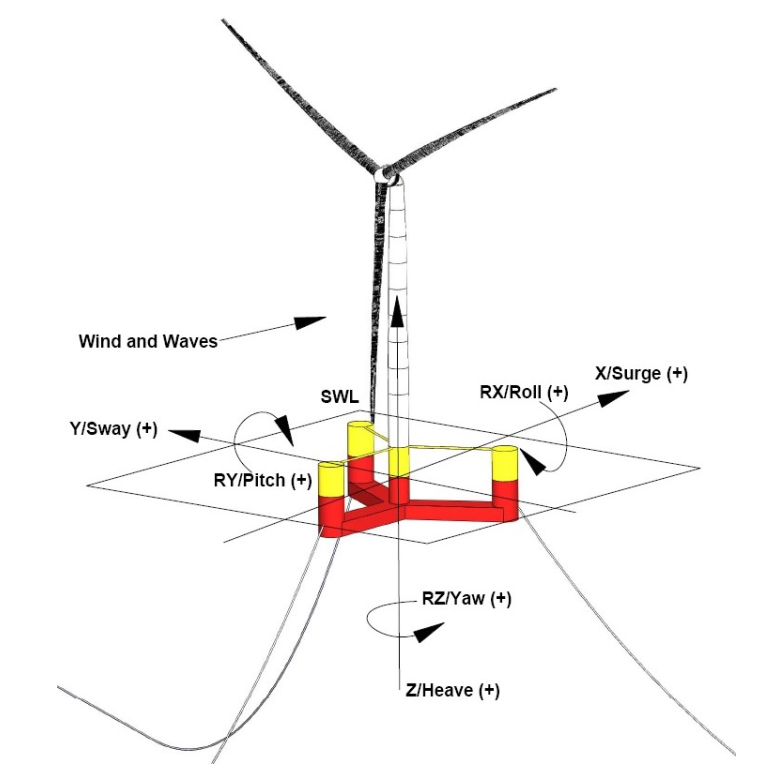
\includegraphics[width=0.55\linewidth]{Graphics/FOWTcoordinates.png}
	\caption{The 6 degrees of freedom (DOFs) of a floating offshore wind turbine. (This is not the specific WT which is modelled in this report) \cite{Vanelli2021}}
	\label{fig:fowt_coordinates}
\end{figure}
Because of the increased movement and the tower (and possibly blades??) are reinforced to handle the greater loads. One of the large challenges in the FOWT development is handling the negative dampening problem: As the wind is striking the rotor plane the thrust of the wind pitches the WT foundation backwards. The backwards thrust causes the foundation pitch to oscillate thus changing the relative velocity as seen by the rotor. When the turbine moves forward the relative wind speed is higher resulting in a greater torque. The rotor speed controller will pitch the blades out of the wind to decrease the rotation speed but in the process also decreases the thrust. Thus the WT thrusts forwards even faster as a result of the reduced dampening provided by the higher pitch angle.




\subsection{Problem definition}
Can a state-space controller, applied to a linear control model be used to reduce the fore-aft motion of a floating offshore wind turbine?


